\documentclass[10pt, a4paper,openany]{article}
\usepackage[italian]{babel}
\usepackage[T1]{fontenc}
\usepackage[table]{xcolor}
\usepackage{float}
\restylefloat{table,figure}
\usepackage{graphicx}	
\usepackage[utf8]{inputenc}
\usepackage{amsmath}
\usepackage{fancyhdr}
\usepackage{geometry}
\geometry{a4paper,top=2cm,bottom=2cm,left=2.5cm,right=2.5cm,%
	    heightrounded,bindingoffset=5mm}
\usepackage{amssymb}
\usepackage{amsthm}
\usepackage{multicol}
\usepackage{xcolor}
\usepackage{hyperref}
%\usepackage{url}
%inizia qui aggiunta
\usepackage{collcell}
\usepackage{hhline}
\usepackage{pgf}
\usepackage{multirow}

\def\colorModel{hsb} %You can use rgb or hsb

\newcommand\ColCell[1]{
  \pgfmathparse{#1<50?1:0}  %Threshold for changing the font color into the cells
    \ifnum\pgfmathresult=0\relax\color{white}\fi
  \pgfmathsetmacro\compA{0}      %Component R or H
  \pgfmathsetmacro\compB{#1/100} %Component G or S
  \pgfmathsetmacro\compC{1}      %Component B or B
  \edef\x{\noexpand\centering\noexpand\cellcolor[\colorModel]{\compA,\compB,\compC}}\x #1
  } 
\newcolumntype{E}{>{\collectcell\ColCell}m{0.4cm}<{\endcollectcell}}  %Cell width
\newcommand*\rot{\rotatebox{90}}
%Finisce qua
\DeclareMathOperator*{\argmax}{arg\,max}
\begin{document}
\begin{center}
\textbf{{La demenza senile: valutazione da un punto di vista statistico}}
\end{center}

\begin{center}
Vittorio Bomba, Federico Luzzi,  Marco Peracchi, Christian Uccheddu
\end{center}

\hrule
\vspace{0.3cm}

\begin{center}\textbf{{Sommario}}
\end{center}

La demenza senile è un disturbo delle funzioni intellettive legate alla memoria, al linguaggio e al pensiero che colpisce individui in età avanzata, ovvero soggetti con un età superiore ai sessant'anni. Tale malattia accoglie al suo interno diverse sfumature, che tengono conto della sua natura e delle sue cause, di seguito ne verranno indicate alcune:
\begin{itemize}
    \item Demenza degenerativa, che include l'Alzheimer, attribuibile a difetti genetici
    \item Demenza vascolare, derivante dal susseguirsi di microinfarti ripetuti che distruggono il tessuto cerebrale
    \item Demenza reversibile, derivante da disfunzioni che possono essere corrette
\end{itemize}
Data la definizione molto generica e qualitativa di demenza, non esistono parametri clinici che possano univocamente certificare il disturbo, che viene attestato dal medico sulla base di esami medici e parametri ambientali. La necessità di valutare accuratamente la serietà di questa  disfunzione ha portato alla creazione di un test, noto come CDR (Clinical Dementia Rating), una valutazione numerica assegnata dal medico che riporta la gravità della demenza sulla base di un'intervista strutturata per verificare la smemoratezza del paziente. \\
L'obiettivo del progetto è stimare il valore del CDR sulla base di modelli di machine learning, questo potrebbe essere utile per sostituire l'intervista al paziente o per fungere da supporto al medico nell'assegnazione del valore CDR. 
\vspace{0.3cm}
\hrule
\begin{multicols}{2}
\tableofcontents
\section{Premessa}
Il dataset oggetto del nostro studio si chiama \textit{MRI and Alzheimers}, preso dalla piattaforma online di condivisione dati Kaggle, in particolare il file $oasis\_longitudinal.csv$. Il campionamento effettuato è di tipo longitudinale:  uno studio condotto in un determinato tempo, prendendo una porzione di popolazione.
Esso raccoglie i dati clinici di 150 soggetti di età compresa tra i 60 e i 96 anni con una demenza senile \textit{sospetta}. Ciascun record rappresenta una visita effettuata su un soggetto, almeno 2 visite per soggetto.


\section{Descrizione Dataset}
Il dataset è composto da 373 record organizzati in 15 colonne, ognuna delle quali esplicita un attributo della tupla. Di seguito la loro descrizione:
\begin{itemize}
\setlength\itemsep{0.2em}
    \item Subject ID: sequenza di caratteri alfanumerici che identifica il paziente
    \item MRI ID: numero identificativo della risonanza magnetica eseguita sul paziente. Compare come il Subject ID seguito dal numero della risonanza magnetica
    \item Visit: numero della visita dell'individuo
    \item MR delay: tempo intercorso in secondi tra l'iniezione del liquido di contrasto e l'esecuzione della risonanza
    \item M/F: genere del paziente (maschio o femmina)
    \item Hand: mano dominante del soggetto (tutti i soggetti interessati usano la mano destra)
    \item Age: età del paziente
    \item EDUC: anni di istruzione
    \item SES: status socioeconomico assegnato dall'Hollingshead Index of Social Position sulla base di un punteggio che va da 1 (più alto status) a 5 (più basso status)
    \item MMSE: Mini-Mental State Examination, un test neuropsicologico costituito da 30 domande utilizzate per verificare lo stato cognitivo. Va da 1 (peggior stato) a 30 (miglior stato). Con un punteggio inferiore a 24 il paziente presenta indebolimento cognitivo ma non necessariamente demenza;
    \item eTIV: estimated Intracranical Volume, stima del volume intracranico in cm$^3$
    \item nWBV: normalized Whole-Brain Volume, espresso come percentuale del volume del cervello in rapporto con il volume intracranico (eTIV)
    \item ASF: Atlas Scaling Factor, determinante della matrice di trasformazione tra lo spazio della MRI e la mappa utilizzata per strutturare il cervello. In pratica restituisce il raporto fra la misura del volume dell'immagine e della mappa. 
    \item CDR: Clinical Dementia Rating, scala numerica che identifica la gravità della demenza. In particolare si ha 0 per un paziente normale, 0.5 per dubbia demenza, 1 per lieve demenza, 2 per moderata demenza, 3 per grave demenza. Infine 4 e 5 rappresentano i casi più gravi in assoluto.
    \end{itemize}

Nel nostro caso abbiamo la seguente distribuzione di CDR:    
\begin{figure}[H]
	\centering
	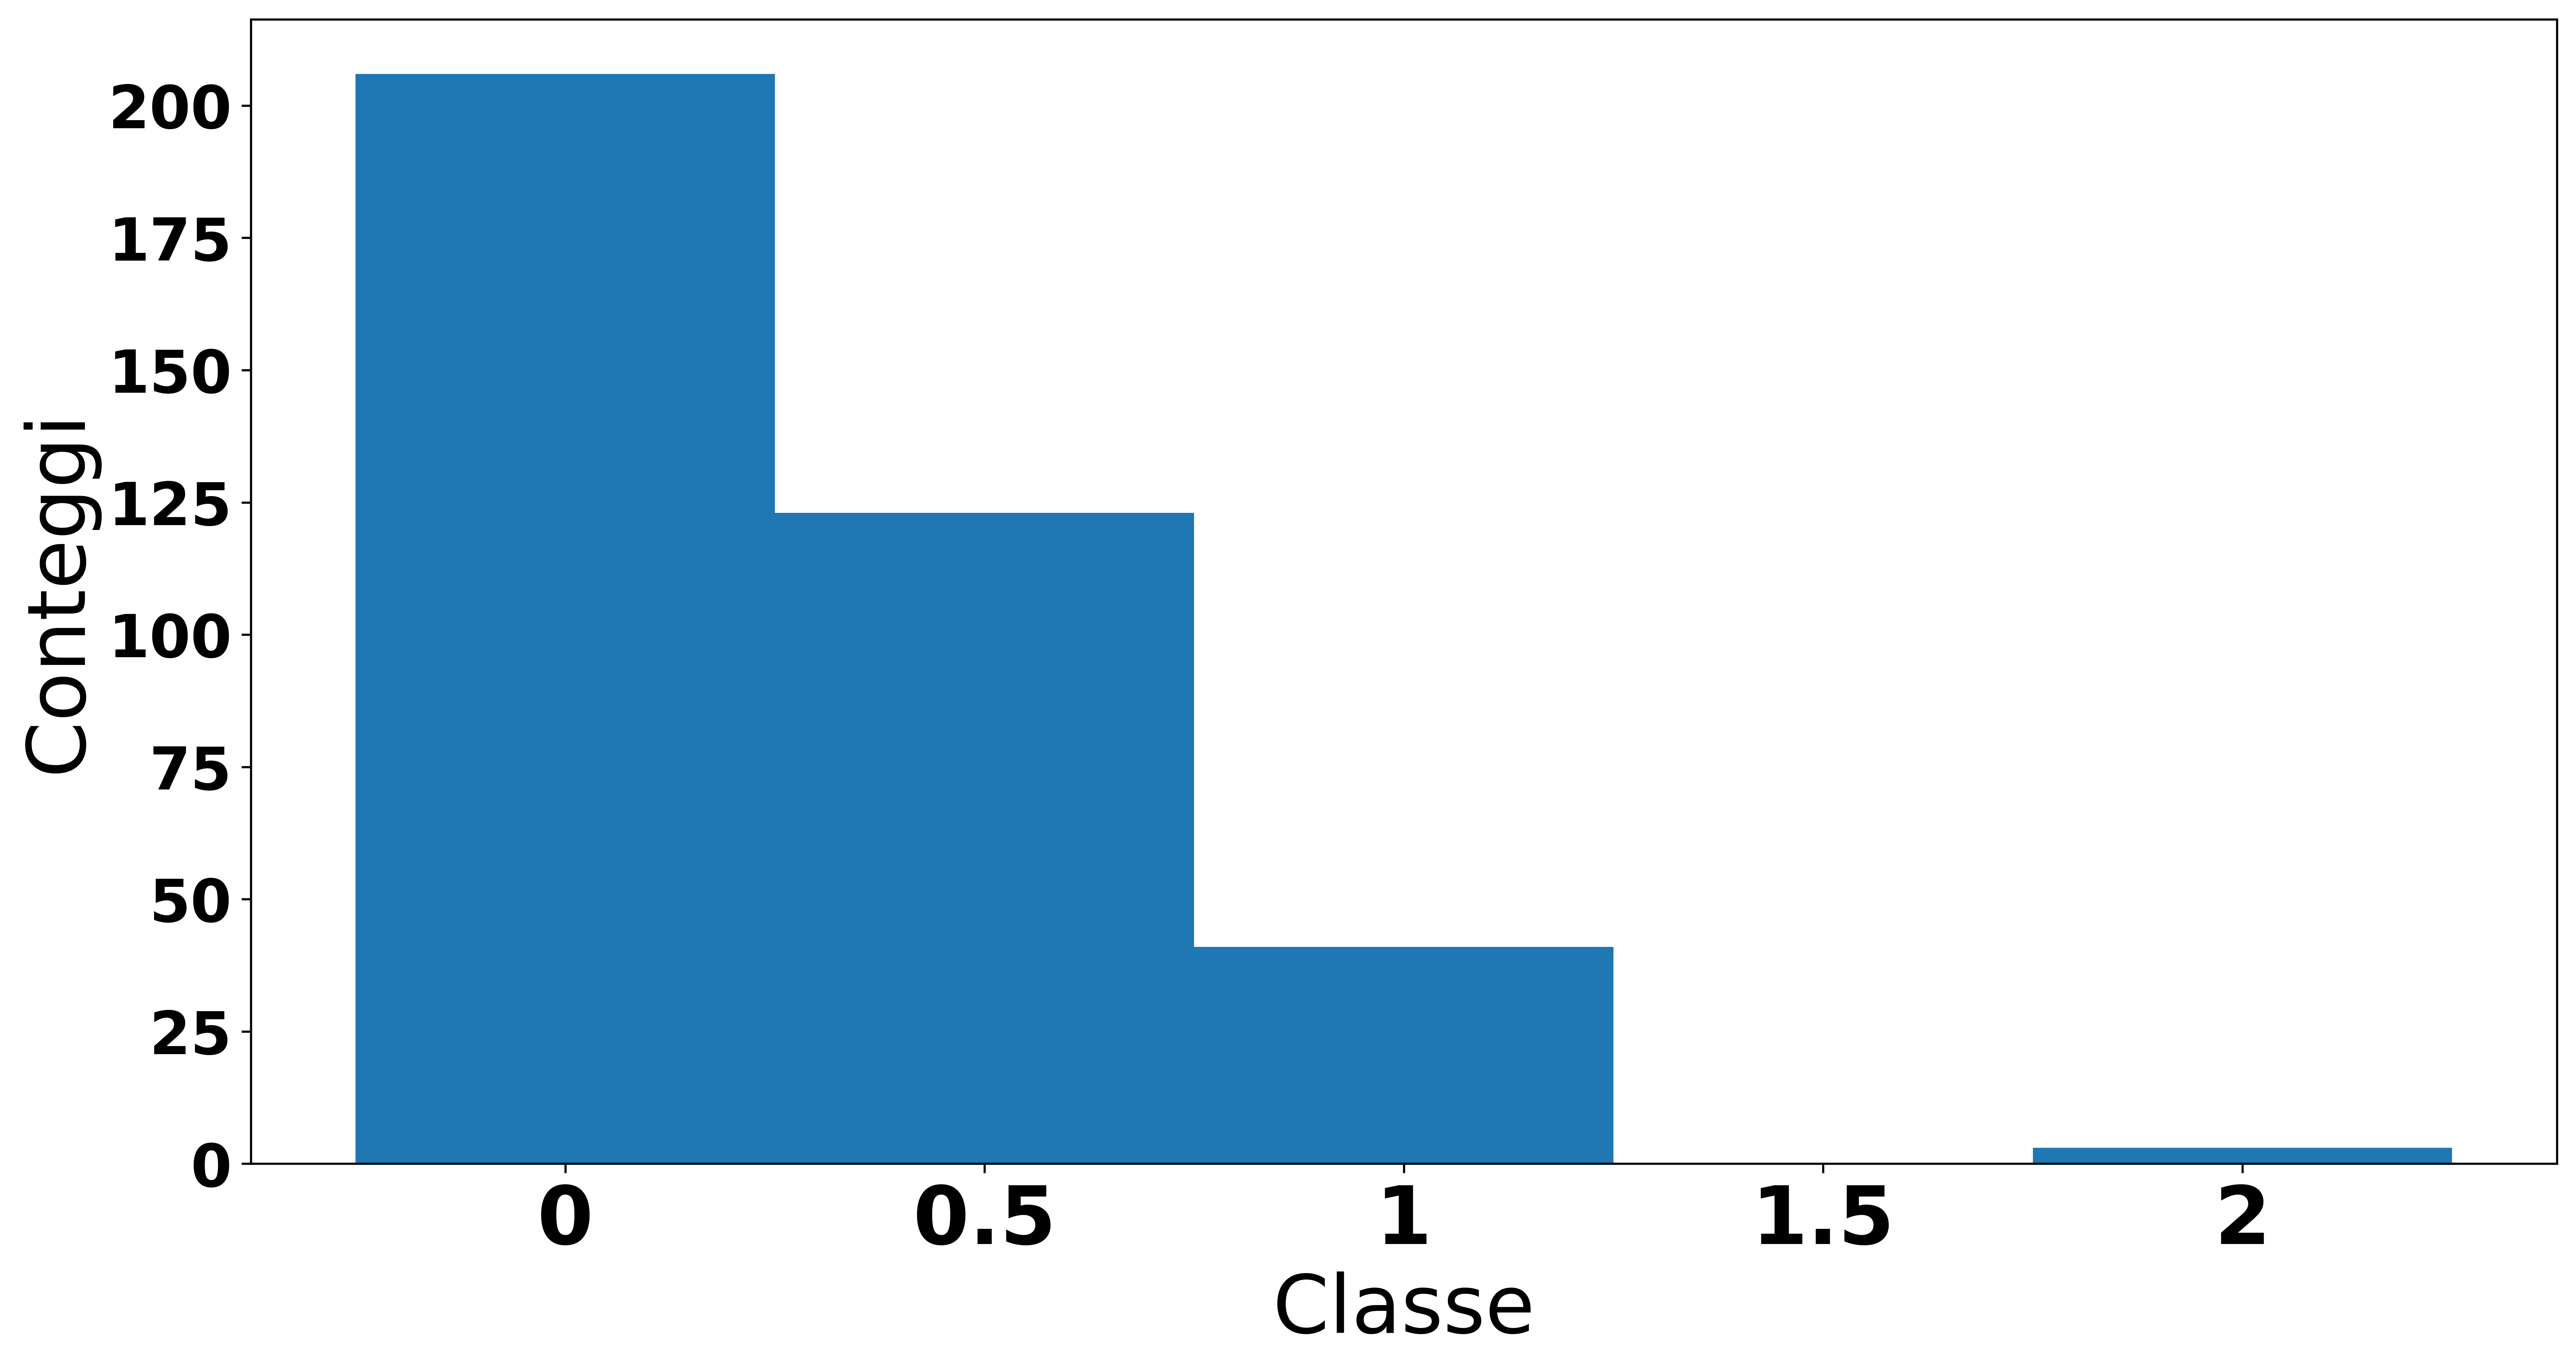
\includegraphics[height=0.55 \linewidth]{bar_plot.png}
	\caption{I valori più bassi sono molto più numerosi e non è presente la classe 1.5}
\end{figure}
    
    
    
    
    
\section{Data Pre-processing} (correlazioni tra variabili e esclusione variabili inutili) 
Missing values
partizionamento \\
Nel lavoro di data-preprocessing ci siamo curati di riempire i valori delle celle mancanti, eliminare le correlazioni fra le variabili  ed escludere le variabili inutili

\subsection{Missing values}
Il dataset presenta 19 valori mancanti alla voce SES e 2 alla voce MMSE. La trattazione di tali valori è stata affrontata in modo differente:
\begin{itemize}
    \item SES: qui i valori mancanti sono stati sostituiti dall'interpolazione lineare con i dati presenti dell'attributo in questione. Questo per mantenere la distribuzione dei dati piuttosto omogenea.
    \item MMSE: in questo caso le righe corrispondenti ai valori mancanti sono state scartate. Considerando che l'MMSE si basa su un questionario scritto individuale ed è quindi una variabile difficile da essere predetta sulla base dei risultati degli altri pazienti. Inoltre i record scartati sono solo due, dunque si assume non inficino visibilmente sui risultati finali.
\end{itemize}
 
\subsection{Correlazione fra le variabili}
Alcuni attributi del dataset risultano essere legati tra di loro. Vista la definizione di eTIV, nWBV e ASF un legame tra di essi sembra suggerito. Analizzando gli attributi si può notare una correlazione quasi lineare tra ASF e il volume intracranico, in quanto all'aumentare del volume intracranico diminuisce il fattore di scala. La spiegazione risiede nel fatto che aumentando il volume intracranico aumenta, di conseguenza, anche il possibile volume del cervello, causando quindi la diminuzione del fattore di scala tra il cervello del paziente e quello standard, ovvero l'ASF.
La percentuale di volume cerebrale (nWBV), invece, non risulta avere connessioni con l'ASF. Infatti la percentuale è insensibile alle variazioni di grandezza del cranio.
Le precedenti considerazioni ci portano a escludere l'attributo ASF dai modelli.

\begin{figure}[H]
    \centering
    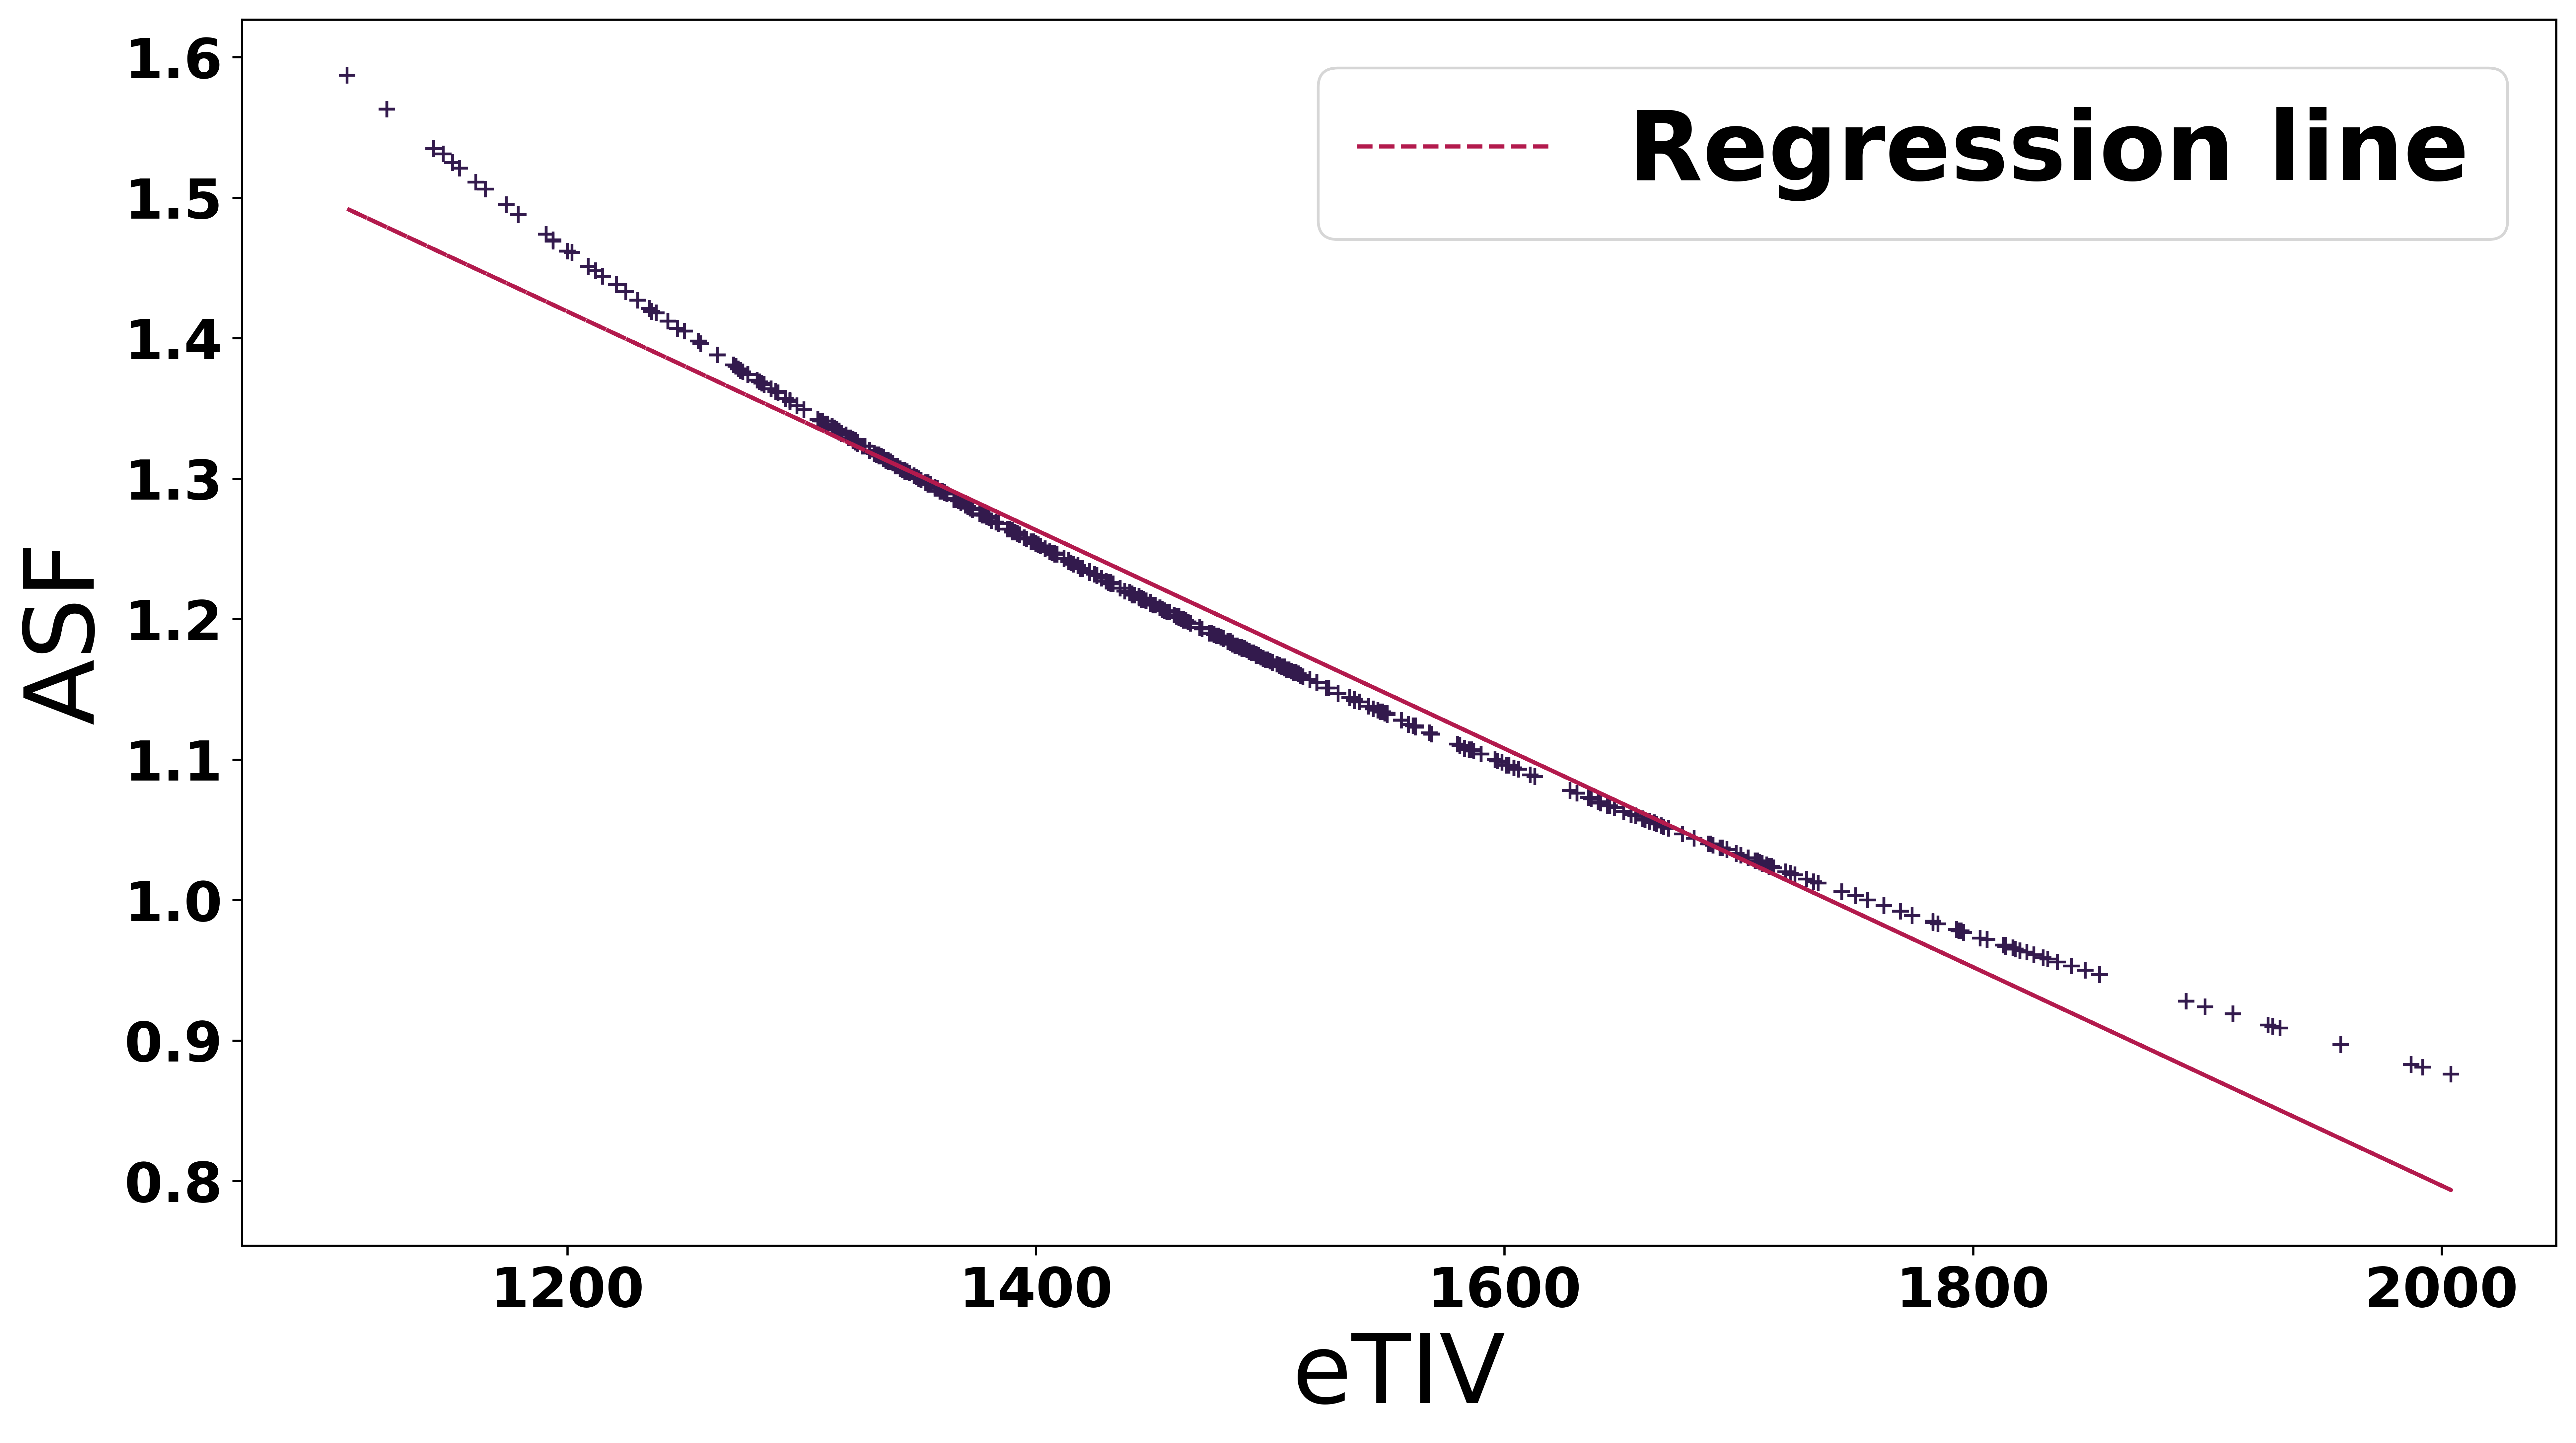
\includegraphics[height=0.55 \linewidth]{eTIV_ASF.png}
    \caption{Il grafico mostra sulle ascisse il volume intracranico (eTIV) e sulle ordinate l'Atlas Scale Factor (ASF)}
    \label{fig:conf sperimentale}
\end{figure}


%Gli unici parametri correlati sono l'eTIV e ASF. Infatti il primo restituisce il volume intracranico, il secondo il rapporto fra il cervello del paziente e il volume intracranico e il terzo rappresenta il fattore di scala fra il cervello del paziente e il cervello "standard" nell'atlante scelto. Dalla conoscenza di due fra i tre parametri possiamo quindi ricavare il terzo, per eliminare questa dipendenza scegliamo quindi di eliminare l'attributo ASF.










\section{Modelli}
Data la natura discreta della variabile di target CDR abbiamo deciso di affrontare la criticità come un problema di classificazione.
Sono stati valutati diversi modelli appartenenti a varie tecniche di classificazione per identificare la più adatta al nostro caso. Di seguito vengono elencati i modelli provati.
\begin{itemize}
\setlength\itemsep{0.2em}
    \item Tecniche Euristiche (decision tree): Random Forest, J48
    \item Tecniche Regression Based: Regressione Logistica
    \item Tecniche di Separazione: Multi Layer Perceptron
    \item Tecniche Probabilistiche: Naive Bayes, Naive Bayes Tree
\end{itemize}

\subsection{Tecniche Euristiche} 

\paragraph{J48:} è una tecnica basata sul concetto di albero decisionale, in cui la particolarità è quella di riuscire a classificare anche dati nominali. Nella nostra implementazione abbiamo impostato un fattore di confidenza di 0.25 e un numero di fold pari a 3.

\paragraph{Random Forest:} La Random Forest è una tecnica basata su comitati di alberi decisionali. Nella nostra implementazione sono stati inseriti 10 alberi con un fattore di confidenza di 0.25 e 3 folds.

\subsection{Tecniche regression based}

\paragraph{Regressione logistica:}è una tecnica di classificazione basata sulla regressione, viene infatti calcolata la probabilità a posteriori che la variabile target restituisca il valore di input. La formula usata dal nodo Knime per calcolare la probabilità associata alla classe j-esima, a meno dell'ultima classe, è la seguente:
\[P_j(X_i) = \frac{e^{X_iBj}}{\sum_{j=1}^{k-1}e^{X_iBj}+1}\]
Mentre la probabilità associata all'ultima classe è espressa come:
\[1- \sum_{j=1}^{k-1}P_j(X_i)\]
Per trovare la regressione migliore è necessario minimizzare la funzione Likelihood relativa a questa distribuzione di probabilità.

\subsection{Tecniche di separazione}

\paragraph{MLP (Multi Layer Perceptron):} è un modello di classificazione basato sulla separazione dello spazio degli attributi, più precisamente consiste in neuroni che comunicano in modo feedforward dalle variabili di input alla variabile di classe. In particolare è stata predisposta una rete a \textbf{2 strati nascosti} con \textbf{5 neuroni per strato.} Questa scelta di parametri è dovuta ad una serie di prove empiriche effettuate per l'ottimizzazione della classificazione. 

\subsection{Tecniche probabilistiche}

\paragraph{Naive Bayes:} è una tecnica di classificazione basata sull'applicazione del teorema di Bayes; un classificatore di  Bayes combina il modello con una regola decisionale. Questo usa la regola per assegnare  alla variabile $\hat{y}$ l'indice di classe $C_k$ da predire. Nel metanodo inserito in Knime abbiamo usato la regola che massimizza la funzione che calcola la probabilità di ottenere la predizione $\hat{y}=C_k$ dato il record $\{x_i\}$, ovvero la \textbf{MAP decision rule}: 
\[\hat{y} = \argmax_{k \in \{k_1, k_1,...,k_n\}} (p(C_k)\prod\limits_{i = 1}^{n}p(x_i|C_k)) \]
\paragraph{Naive Bayes tree:} è un modello che genera un albero decisionale in cui è implementato un classificatore di Bayes in corrispondenza dei nodi.
\section{Elaborazione e interpretazione dei dati}
%Io farei notare di più i nomi degli indici in modo che saltino all'occhio nella lettura (con un grassetto o usare il paragraph) (fede)
Per valutare i risultati sono stati utilizzati diversi indici, primo fra tutti l'\textit{accuracy}. L'accuracy misura l'affidabilità del modello a predire risultati corretti su nuovi dati. Per calcolare l'accuracy sul dataset $D$, con $n$ entrate, a predire la variabile $y_i$ dati i valori $\{x_i\}$ ($f(x_i)$ rappresenta la previsione) si sfrutta la seguente formula:
\[acc(D) = 1 - \frac{1}{n}\sum_{j=1}^{n}L(y_i,f(x_i))\]
L rappresenta la  \textit{loss function}, funzione che assegna valore 1 se $y_i \neq f(x_i)$ (cioè la predizione è errata) e 0 viceversa. Si può notare quindi che all'aumentare delle previsione errate diminuisce il valore dell'accuracy.
I modelli utilizzati restituiscono la matrice di confusione. Questa contiene al suo interno diversi valori, nel nostro caso i valori di CDR che potevano essere predetti erano 0, 0.5, 1 e 2. Un esempio di matrice di confusione appare così:

\newcommand\items{4}   %Number of classes
\arrayrulecolor{white} %Table line colors
\begin{center}
\noindent\begin{tabular}{cc*{\items}{|E}|}
\multicolumn{1}{c}{} &\multicolumn{1}{c}{} &\multicolumn{\items}{c}{CDR} \\ \hhline{~*\items{|-}|}
\multicolumn{1}{c}{} & 
\multicolumn{1}{c}{} & 
\multicolumn{1}{c}{0} & 
\multicolumn{1}{c}{0.5} & 
\multicolumn{1}{c}{1} &
\multicolumn{1}{c}{2} \\ \hhline{~*\items{|-}|}
\multirow{\items}{*}{\rotatebox{90}{$CDR_{pred}$}} 
&0  & 60 & 8 & 0 & 0 \\ \hhline{~*\items{|-}|}
&0.5 & 12 & 18 & 6 & 0 \\ \hhline{~*\items{|-}|}
&1  &  1 & 1 & 10 & 0\\ \hhline{~*\items{|-}|}
&2  & 0 & 1 & 0 & 0\\ \hhline{~*\items{|-}|}
\end{tabular}
\end{center}

Sulla diagonale si possono notare i valori previsti correttamente dal modello, mentre gli altri rappresentano valori previsti in maneira scorretta.

La accuracy è calcolata sommando i valori sulla diagonale e dividendoli per il totale. 

Il secondo indice utilizzato è la \textit{precision}. Viene definita come il rapporto tra i valori predetti correttamente della variabile che consideriamo diviso il numero di valori totali che appaiono nel dataset per quella variabile. Per esempio la precision della variabile 0.5 è:
\[P(0.5) = \frac{18}{12+18+6} = 0.50\]

Un altro indice sfruttato è la \textit{recall}. La recall viene calcolata sfruttando di nuovo il numero di valori predetti correttamente per la variabile considerata diviso il numero di valori totali predetti dal modello per quella variabile. Nuovamente riproponiamo come esempio la variabile 0.5, per cui la recall sarà:
\[R(0.5) = \frac{18}{8+18+1+1} = 0.64\]

L'ultimo indice che abbiamo sfruttato è la \textit{F-measure}. Viene calcolato sfruttando gli indici elencati precedentemente:
\[F = \frac{2\cdot r \cdot p}{r + p}\]
Valori elevati della F-measure indicano valori elevati di entrambi recall e precision. Pre concludere l'esempio portato precedentemente otteniamo:
\[F(0.5) = \frac{2 \cdot 0.50 \cdot 0.64}{0.50 + 0.64}=0.56\]
Per calcolare il valore di un indice complessivo di ogni modello abbiamo preso quindi la media aritmetica degli indici calcolati sulle singole classi di quel modello nel modo seguente:
\[I_{model} = \frac{I(0) + I(0.5)+ I(1) + I(2)}{4}\]
Con I: accuracy, F-Measure, recall, precision.

In questo modo è possibile confrontare i modelli.

\subsection{Holdout}
La tecnica di Holdout consiste nel dividere il dataset in due partizioni usando un campionamento stratificato, ovvero mantenendo le proporzioni degli attributi delle partizioni uguali alle proporzioni tra gli attributi nel dataset di partenza. Questo metodo permette di sfruttare una parte del dataset come \textit{train}, per addestrare il codice, e una parte come \textit{test}, per valutare le predizioni fatte. Le misure di performance vengono eseguite sulla partizione di test. 
La problematica principale di questa tecnica è la dipendenza dell'accuracy dal partizionamento iniziale. Determinate divisioni potrebbero sovrastimare o sottostimare l'accuracy.


\begin{table}[H]
\tabcolsep=0.10cm
\small
    \centering
    \begin{tabular}{ccccc}
     Modello & Recall & Precision & F-Measure & Accuracy  \\
     \hline
     MLP & 0.511 & 0.512 & 0.504 & 0.748 \\
     NB & 0.471 & 0.533 & NaN & 0.756 \\
     NBTree & 0.536 & 0.522 & 0.527 & 0.748 \\
     J48 & 0.439 & 0.443 & 0.440 & 0.691 \\
     RF & 0.499 & 0.509 & 0.503 & 0.740 \\
     Log & 0.525 & 0.573 & NaN & 0.780 \\
     \hline
    \end{tabular}
    \caption{Misure di valutazione relative ai diversi modelli con il metodo holdout}
\end{table}

INSERIRE INTERPRETAZIONE DEI RISULTATI
\subsection{Iterated Holdout}

La tecnica dell'iterated holdout consiste nell'iterare il metodo descritto nel paragrafo precedente. In tal modo si cerca di superare l'incoveniente della dipendenza dal partizionamento eseguendo più volte esso in maniera sempre casuale. La accuracy è calcolata semplicemente con una media di tutti i risultati ottenuti dai vari partizionamenti. La criticità del metodo risiede nell'impossibilità di controllare le divisioni del dataset, che in caso di valori molto sbilanciati potrebbe portare a risultati poco sensati di accuracy.


\begin{table}[H]
\tabcolsep=0.10cm
\small
\begin{tabular}{ccccc}

     Modello & Recall & Precision & F-Measure & Accuracy  \\
     \hline
     MLP & 0.489 & 0.500 & 0.485 & 0.722 \\
     NB & 0.486 & 0.516 & 0.482 & 0.728 \\
     NBTree & 0.455 & 0.481 & 0.453 & 0.689 \\
     J48 & 0.464 & 0.472 & 0.462 & 0.684 \\
     RF & 0.492 & 0.506 & 0.498 & 0.733 \\
     Log & 0.473 & 0.485 & 0.464 & 0.711 \\
     \hline
\end{tabular}
\caption{Misure di valutazione relative ai diversi modelli con il metodo iterated holdout}
\end{table}

INSERIRE INTERPRETAZIONE DEI RISULTATI

\subsection{Cross-validation}
La cross-validation utilizza un metodo leggermente diverso dall'iterated holdout. Il dataset viene suddiviso in diverse parti, di cui una verrà utilizzata come test e le altre come train. La accuracy viene calcolata nuovamente con una media.
La cross-validation permette inoltre di controllare il metodo di partizionamento, nel nostro caso abbiamo utilizzato un campionamento stratificato, a causa dei valori abbastanza sbilanciati della classe CDR. In tal modo abbiamo potuto garantire all'interno di ogni partizione la giusta proporzione tra i vari punteggi.

\begin{table}[H]
\tabcolsep=0.10cm
\small
\begin{tabular}{c c c c c}
     Modello & Recall & Precision & F-Measure & Accuracy  \\
     \hline
     MLP & 0.457 & 0.499 & 0.471 & 0.698 \\
     NB & 0.498 & 0.541 & NaN & 0.741 \\
     NBTree & 0.456 & 0.487 & 0.466 & 0.722 \\
     J48 & 0.433 & 0.455 & 0.441 & 0.674 \\
     RF & 0.487 & 0.499 & 0.492 & 0.736 \\
     Log & 0.493 & 0.529 & Nan & 0.744 \\
     \hline
\end{tabular}
\caption{Misure di valutazione relative ai diversi modelli con il metodo cross validation}
\end{table}

INSERIRE INTERPRETAZIONE DEI RISULTATI

\subsection{Feature selection}

Con l'obiettivo di migliorare le performance dei modelli e l'interpretabilità degli stessi, vengono effettuate delle feature selection. Si applica un'ottimizzazione di tipo \textbf{Wrapper}: un classificatore estrae gli attributi rilevanti con i quali viene trainato il nuovo modello. Si utilizza lo stesso classificatore come wrapper e vengono provati tutti i modelli definiti in precedenza. Il dataset viene suddiviso inizialmente in du



ACCURACY
\begin{table}[H]
\tabcolsep=0.10cm
\small
\begin{tabular}{c c c c c}
     Modello & Recall & Precision & F-Measure & Accuracy  \\
     \hline
     MLP & 0.518 & 0.556 & 0.529 & 0.780 \\
     NB & 0.471 & 0.520 & 0.479 & 0.740 \\
     NBTree & 0.521 & 0.531 & 0.518 & 0.764 \\
     J48 & 0.484 & 0.494 & NaN & 0.740 \\
     RF & 0.521 & 0.531 & 0.518 & 0.764 \\
     Log & 0.515 & 0.537 & 0.593 & 0.764 \\
     \hline
\end{tabular}
\caption{}
\end{table}

RECALL
\begin{table}[H]
\tabcolsep=0.10cm
\small
\begin{tabular}{c c c c c}
     Modello & Recall & Precision & F-Measure & Accuracy  \\
     \hline
     MLP & 0.527 & 0.544 & 0.529 & 0.772 \\
     NB & 0.478 & 0.536 & 0.490 & 0.748 \\
     NBTree & 0.505 & 0.530 & NaN & 0.764 \\
     J48 & 0.508 & 0.530 & 0.513 & 0.764 \\
     RF & 0.512 & 0.495 & NaN & 0.675 \\
     Log & 0.540 & 0.554 & 0.546 & 0.780 \\
     \hline
\end{tabular}
\caption{}
\end{table}

PRECISION

\begin{table}[H]
\tabcolsep=0.10cm
\small
\begin{tabular}{c c c c c}
     Modello & Recall & Precision & F-Measure & Accuracy  \\
     \hline
     MLP & 0.545 & 0.558 & 0.549 & 0.764 \\
     NB & 0.478 & 0.536 & 0.490 & 0.748 \\
     NBTree & 0.533 & 0.559 & 0.540 & 0.780 \\
     J48 & 0.495 & 0.510 & 0.495 & 0.724\\
     RF & 0.424 & 0.446 & NaN & 0.634 \\
     Log & 0.544 & 0.572 & 0.555 & 0.789 \\
     \hline
\end{tabular}
\caption{}
\end{table}

F-MEASURE

\begin{table}[H]
\tabcolsep=0.10cm
\small
\begin{tabular}{c c c c c}
     Modello & Recall & Precision & F-Measure & Accuracy  \\
     \hline
     MLP & 0.545 & 0.558 & 0.549 & 0.764 \\
     NB & 0.471 & 0.520 & 0.479 & 0.740 \\
     NBTree & 0.505 & 0.530 & NaN & 0.764 \\
     J48 & 0.494 & 0.512 & 0.499 & 0.740 \\
     RF & 0.504 & 0.560 & 0.523 & 0.764 \\
     Log & 0.544 & 0.572 & 0.555 & 0.789 \\
     \hline
\end{tabular}
\caption{}
\end{table}
\section{Conclusioni}
risposta alla domanda di ricerca: siamo riusciti o meno a trovare un buon modello?

miglioramenti futuri: più dati e più casi CDR alto. Cercare di capire come modellare l'alzaimer.
\textbf{QUA FRASE DA CAPIRE DOVE METTERE}
Conseguentemente la variabile CDR (Clinical Dementia Rating), che rappresenta la gravità della demenza (valori alti indicano i casi peggiori), non raggiunge valori superiori a 1, in quanto sarebbero casi accertati e non sospetti. Il modello di machine learning progettato potrebbe, di conseguenza, non essere capace di prevedere casi particolarmente gravi. Tuttavia, si suppone che nei suddetti casi i test per comprendere il grado di demenza rappresenterebbero fattori meno significativi e di minor interesse puramente predittivo.


\begin{thebibliography}{1}
	\bibitem{a:tesi}\href{https://surfer.nmr.mgh.harvard.edu/fswiki/eTIV}{\emph{eTIV-estimated Total Intracranial Volume}}
	\bibitem{b:tesi}\href{https://it.wikipedia.org/wiki/Demenza}{\emph{Demenza}}
	\bibitem{c:tesi}\href{https://it.wikipedia.org/wiki/Mini-Mental_State_Examination}{\emph{Mini-Mental State Examination}}
	\bibitem{d:tesi}\href{https://it.wikipedia.org/wiki/Clinical_Dementia_Rating}{\emph{Clinical Dementia Rating}}
	\bibitem{e:tesi}\href{https://pdfs.semanticscholar.org/f078/58e6d1c1463367e1157f2c127b1d1a4652fd.pdf}{\emph{Analysis of Human Brain MRI}, RICHARD NORDENSKJÖLD}
\end{thebibliography}

\end{multicols}
\end{document}


